%CS51 HW9 Assignment
%Preamble
\documentclass[12pt, letterpaper]{article}
\usepackage[utf8]{inputenc}
\usepackage{graphicx}
\usepackage{comment}
\usepackage{subcaption}
\usepackage[export]{adjustbox}
\usepackage[margin=0.25in]{geometry}
\graphicspath{
{/Users/carterbastian/Desktop/cgood/}{/Users/carterbastian/Desktop/cbad/} }

\usepackage{cleveref}


\title{Control Hazard Demonstration}
\author{Carter J. Bastian \thanks{COSC51 HW9 Q4}}
\date{May 2015}

\begin{document}
\maketitle
% Figure 1 = Step 1 (c1)
\begin{figure}[h]
  % cgood1
  \begin{subfigure}{0.5\textwidth}
    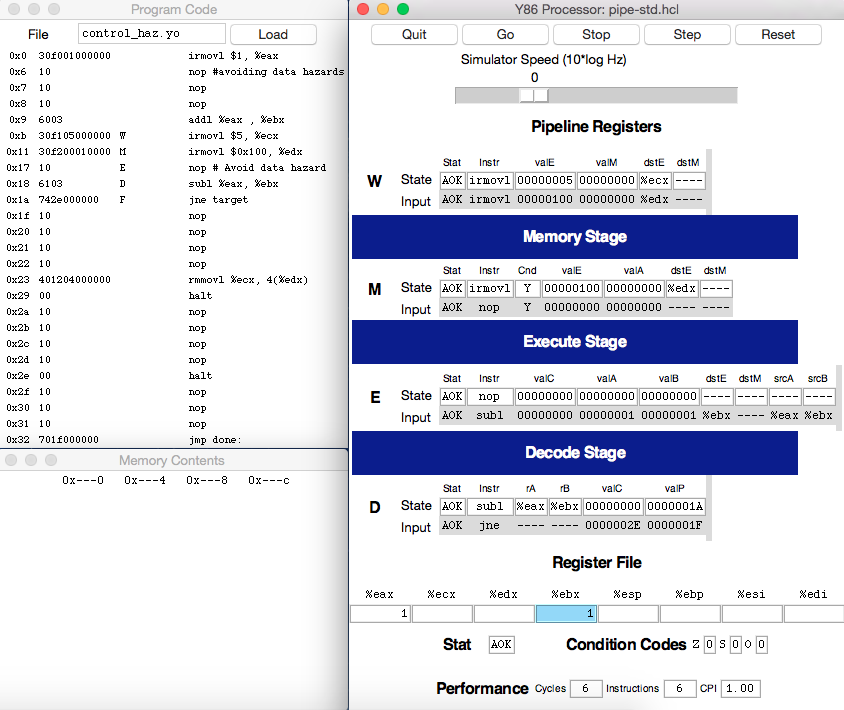
\includegraphics[scale=.35]{cgood1}
    \caption{Correct Implementation (std)}
    \label{fig:cgood1}
    \end{subfigure}
  % cbad1
  \begin{subfigure}{0.5\textwidth}
    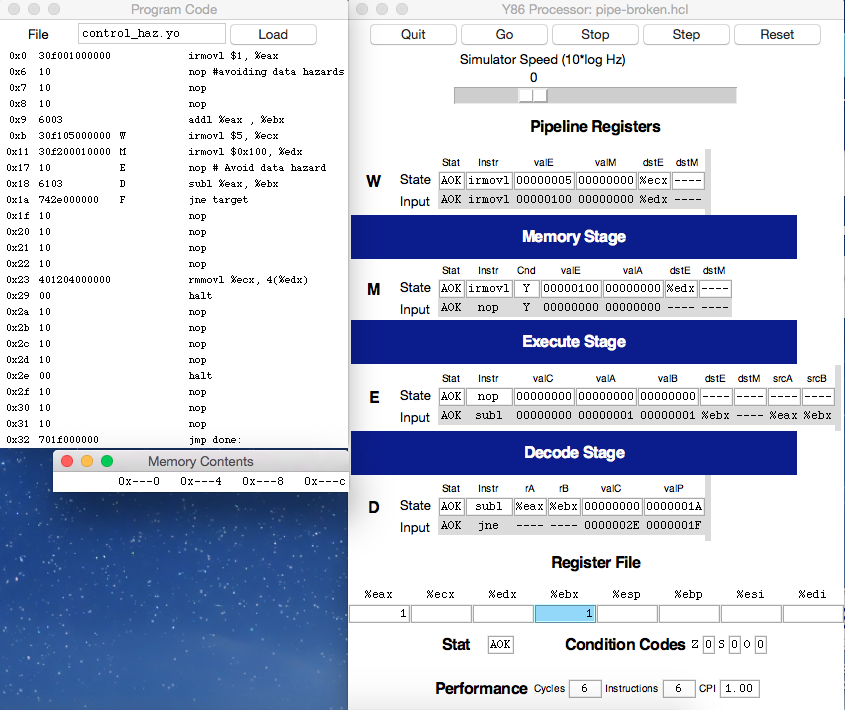
\includegraphics[scale=.35, right]{cbad1}
    \caption{Incorrect Implementation (broken)}
    \label{fig:cbad1}
  \end{subfigure}
  \caption{In this step, the \texttt{jne} instruction has just been
            fetched by the two different versions.}
  \label{fig:c1}
\end{figure}
% Figure 2 = Step 2 (c2)
\begin{figure}[h]
  % cgood2
  \begin{subfigure}{0.5\textwidth}
    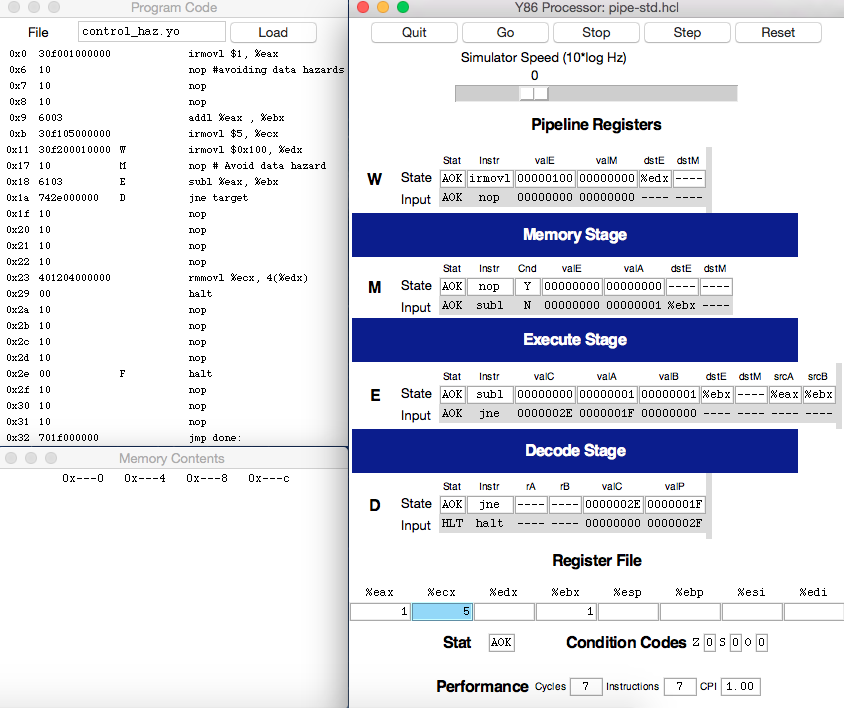
\includegraphics[scale=.35]{cgood2}
    \caption{Correct Implementation (std)}
    \label{fig:cgood2}
    \end{subfigure}
  % cbad2
  \begin{subfigure}{0.5\textwidth}
    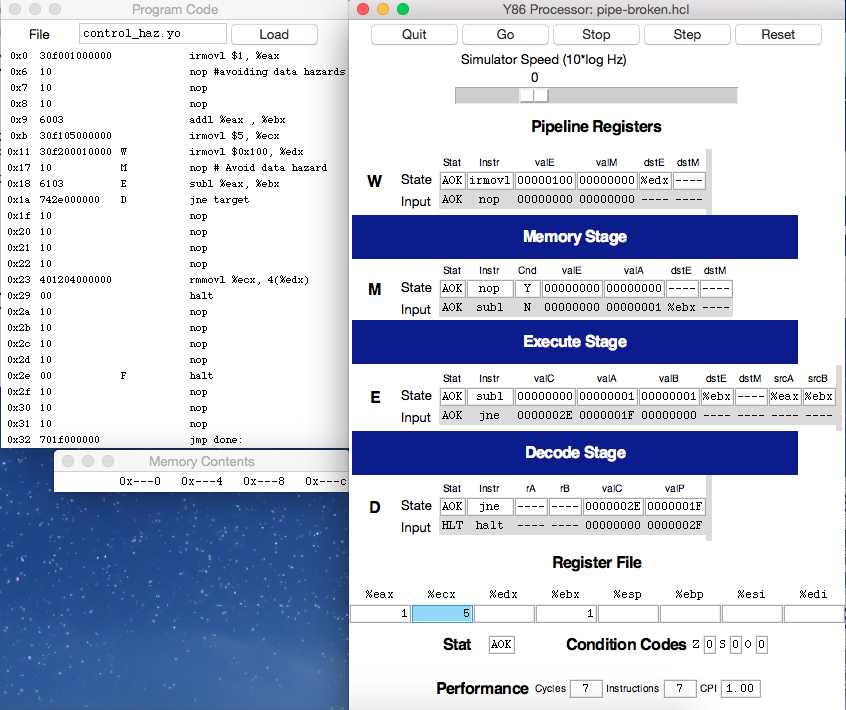
\includegraphics[scale=.35, right]{cbad2}
    \caption{Incorrect Implemenetation (broken)}
    \label{fig:cbad2}
  \end{subfigure}
  \caption{In this step, both implementations predict the conditional
            jump to ``target'' and fetch the \texttt{halt} instruction
            which should not be executed.}
  \label{fig:c2}
\end{figure}
% Figure 3 = Step 3 (c1)
\begin{figure}[h]
  % cgood3
  \begin{subfigure}{0.5\textwidth}
    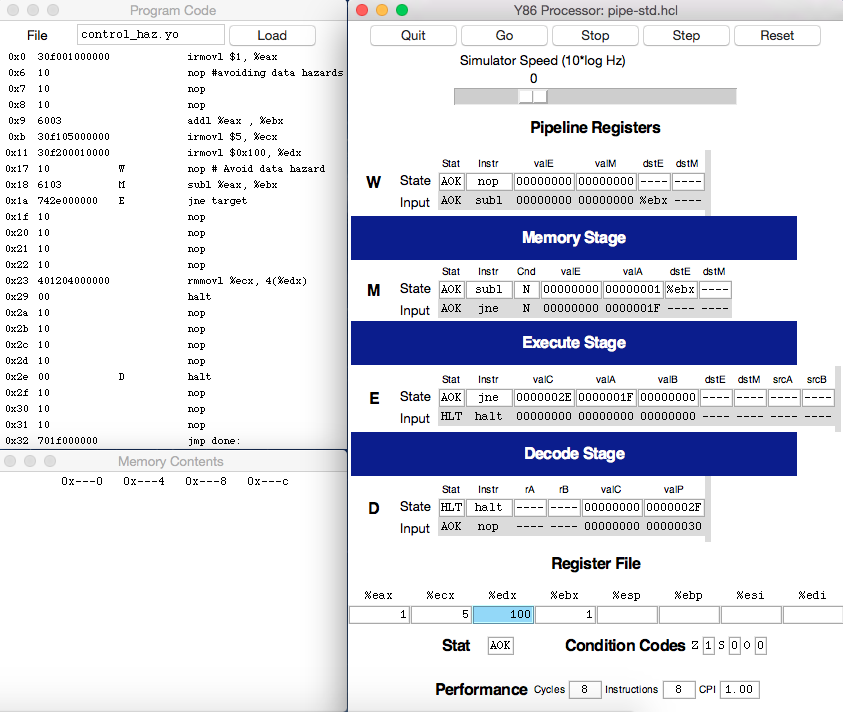
\includegraphics[scale=.35]{cgood3}
    \caption{Correct Implementation (std)}
    \label{fig:cgood3}
    \end{subfigure}
  % cbad3
  \begin{subfigure}{0.5\textwidth}
    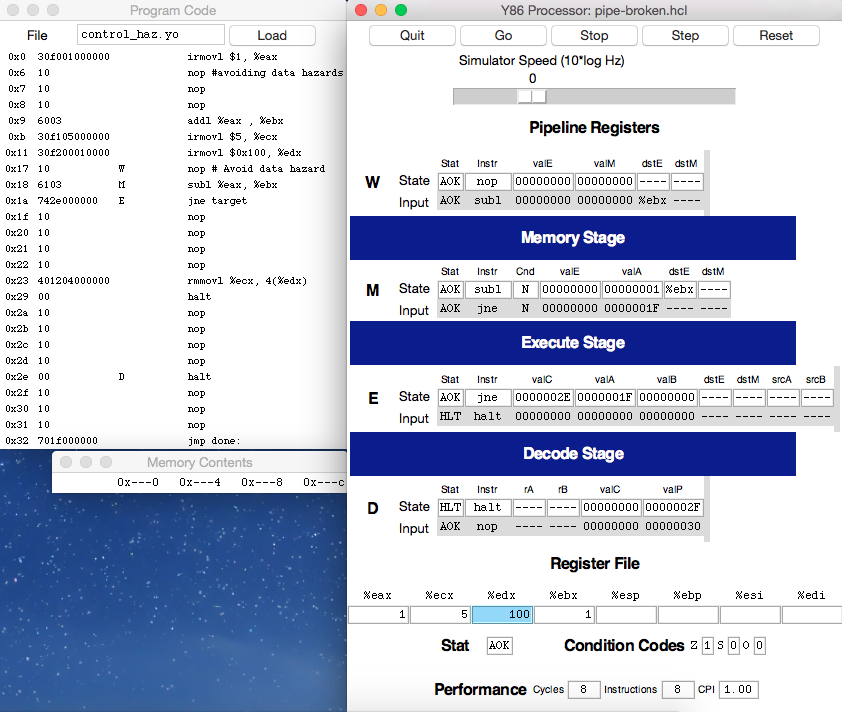
\includegraphics[scale=.35, right]{cbad3}
    \caption{Incorrect Implementation (broken)}
    \label{fig:cbad3}
  \end{subfigure}
  \caption
{The \texttt{jne} instruction reaches the Execute Pipeline Register.
It's now clear that the conditional jump should
not have been taken. However, the ``target's'' \texttt{nop} instruction 
has just been fetched, and the \texttt{halt} instruction has been loaded
into the Decode Pipeline Register.}
  \label{fig:c3}
\end{figure}
% Figure 4 = Step 4 (c4)
\begin{figure}[h]
  % cgood4
  \begin{subfigure}{0.5\textwidth}
    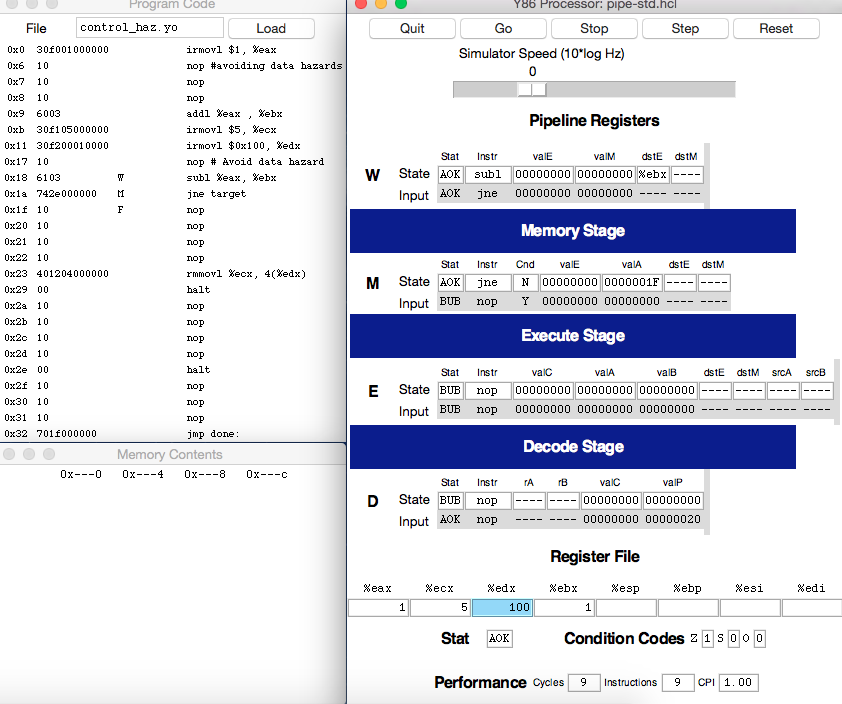
\includegraphics[scale=.35]{cgood4}
    \caption{Correct Implementation (std)}
    \label{fig:cgood4}
    \end{subfigure}
  % cbad4
  \begin{subfigure}{0.5\textwidth}
    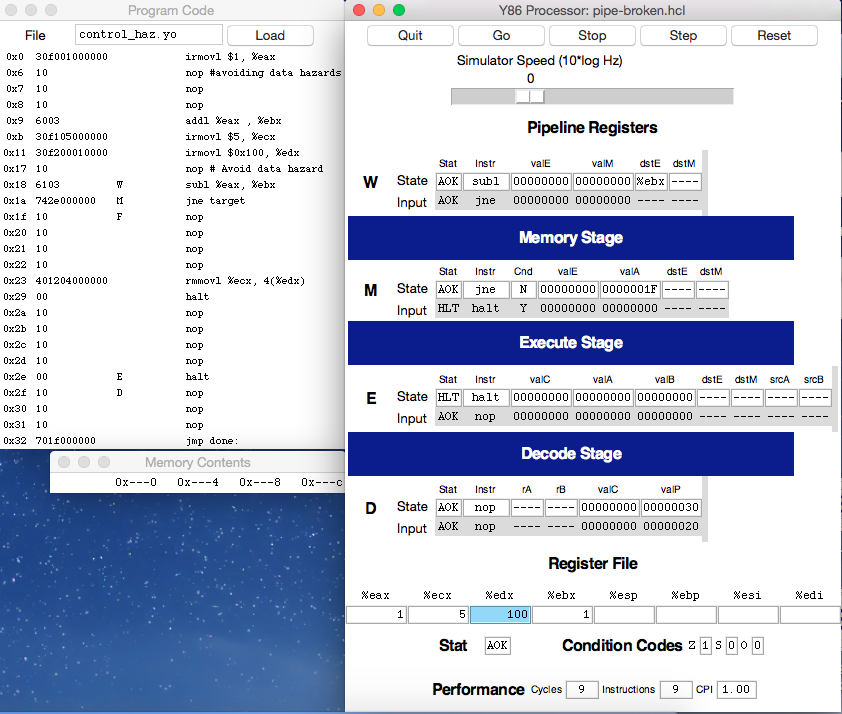
\includegraphics[scale=.35, right]{cbad4}
    \caption{Incorrect Implementation (broken)}
    \label{fig:cbad4}
  \end{subfigure}
  \caption
{This step best illustrates the difference between the two versions. The
correct implementation cancels the two incorrectly-fetched instructions (by
converting them into \texttt{nop bubbles}) and then fetches the next instructions
from the correct location – the ``done'' tag. By doing so, the correct version
mitigates the control hazard. \\
On the other hand, the incorrect version simply fetches the next instruction
from the correct location without cancelling the \texttt{halt} instruction or the
\texttt{nop} instruction, simply progressing them to the Execute and Decode stages
respectively.}
  \label{fig:c4}
\end{figure}
% Figure 5 = Step 5 (c5)
\begin{figure}[h]
  % cgood5
  \begin{subfigure}{0.5\textwidth}
    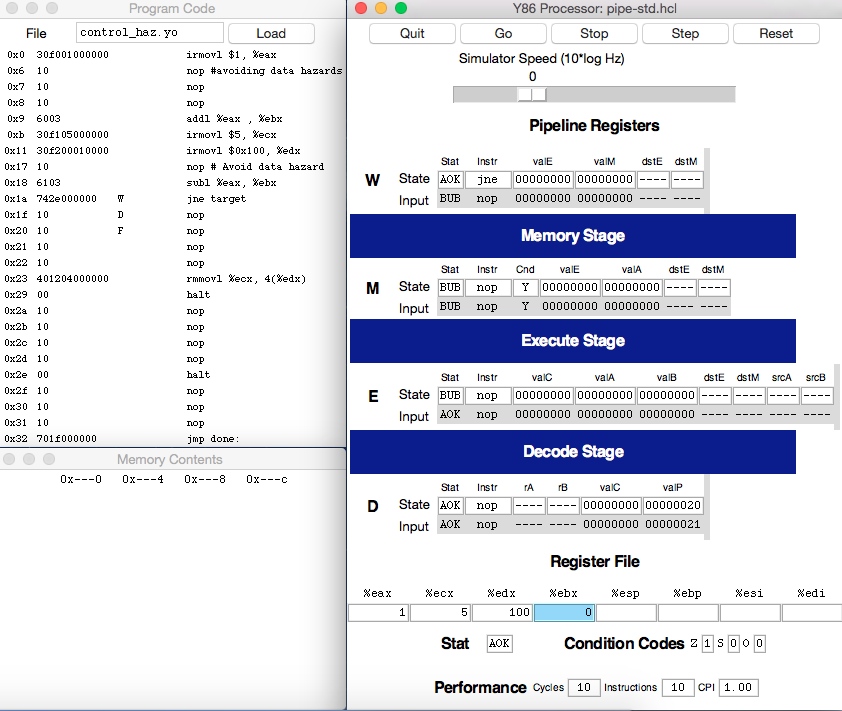
\includegraphics[scale=.35]{cgood5}
    \caption{Correct Implementation (std)}
    \label{fig:cgood5}
    \end{subfigure}
  % cbad5
  \begin{subfigure}{0.5\textwidth}
    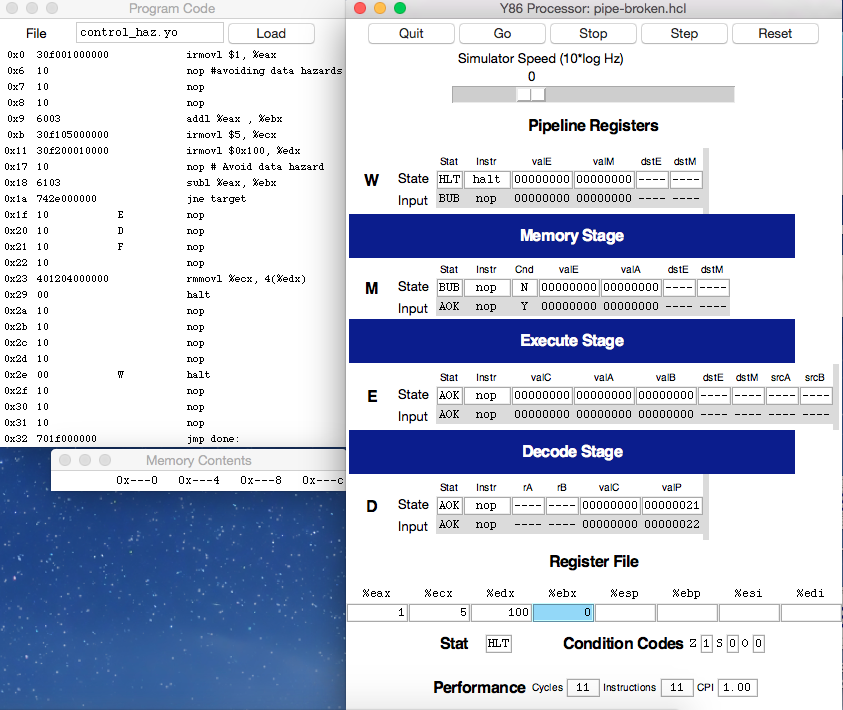
\includegraphics[scale=.35, right]{cbad5}
    \caption{Incorrect Implementation (broken)}
    \label{fig:cbad5}
  \end{subfigure}
  \caption{You can see the invalid instructions progress through the pipeline
stages. You can also see the Correct implementation's \texttt{nop bubbles} move
through the stages and the correct instructions getting fetched.}
  \label{fig:c5}
\end{figure}
% Figure 6 = Step 6 (c6)
\begin{figure}[h]
  % cgood6
  \begin{subfigure}{0.5\textwidth}
    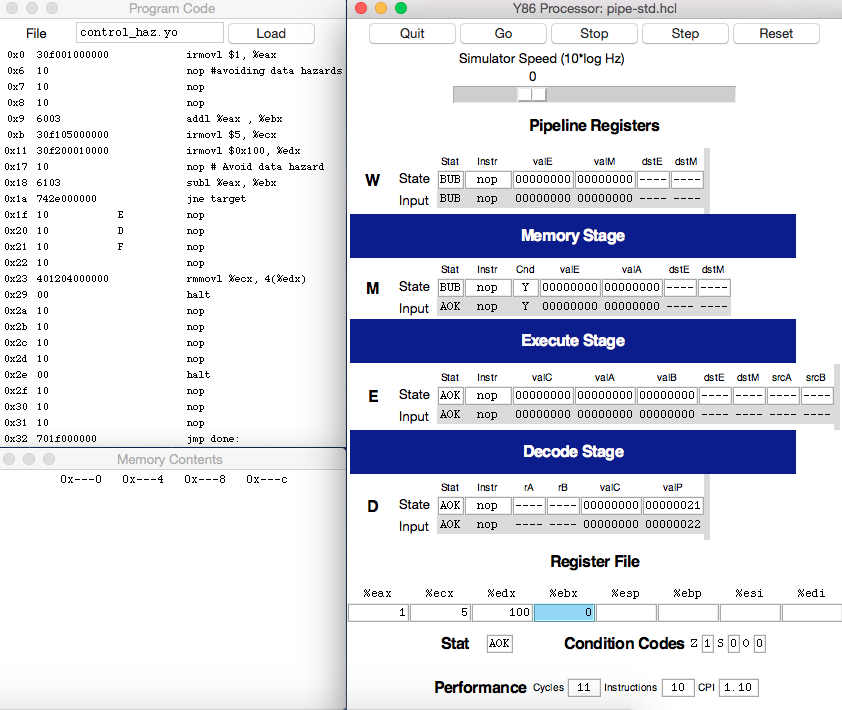
\includegraphics[scale=.35]{cgood6}
    \caption{Correct Implementation (std)}
    \label{fig:cgood6}
    \end{subfigure}
  % cbad6
  \begin{subfigure}{0.5\textwidth}
    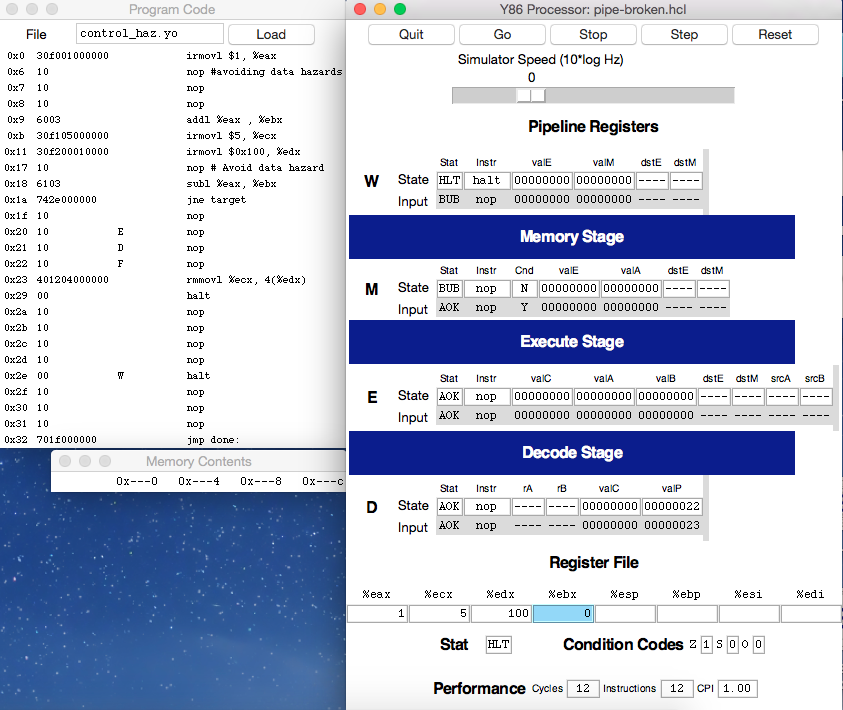
\includegraphics[scale=.35, right]{cbad6}
    \caption{Incorrect Implementation (broken)}
    \label{fig:cbad6}
  \end{subfigure}
  \caption{Both programs have finished processing the \texttt{jne} instruction.
You can see that the correct implementation has successfully continued on to the
right part of the program without allowing the instructions from ``target'' to
change the programmer-visible state. On the other hand, the invalid instruction
is halted and will no longer process instructions. It will never even get to the
rest of the correct instructions in the ``done'' section.}
  \label{fig:c6}
\end{figure}
\begin{figure}[h]
  % cgoodf
  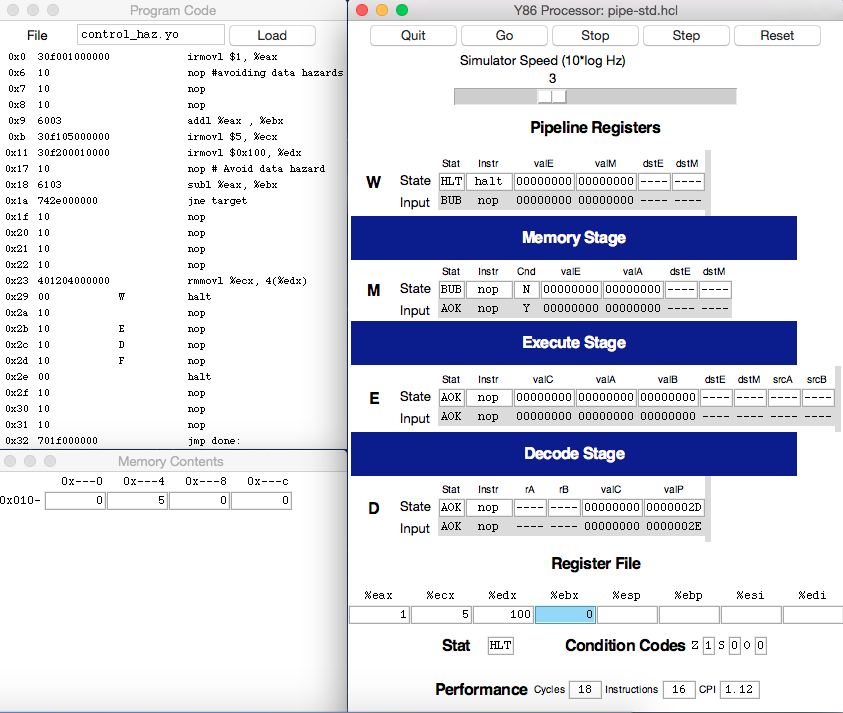
\includegraphics[scale=.35, center]{cgoodf}
  \caption{Here you can see the programmer-visible state from when the Correct
Implementation (std) halts. Compare this to the programmer-visible state from
Figure \ref{fig:c6}: (\subref{fig:cbad6}) and you will see that there are problematic differences caused by the control hazard from control\_haz.ys}
  \label{fig:cgoodf}
\end{figure}
\end{document}
